%
% This is a borrowed LaTeX template file for lecture notes for CS267,
% Applications of Parallel Computing, UCBerkeley EECS Department.
% Now being used for CMU's 10725 Fall 2012 Optimization course
% taught by Geoff Gordon and Ryan Tibshirani.  When preparing 
% LaTeX notes for this class, please use this template.
%
% To familiarize yourself with this template, the body contains
% some examples of its use.  Look them over.  Then you can
% run LaTeX on this file.  After you have LaTeXed this file then
% you can look over the result either by printing it out with
% dvips or using xdvi. "pdflatex template.tex" should also work.
%

\documentclass[twoside]{article}
\setlength{\oddsidemargin}{0.25 in}
\setlength{\evensidemargin}{-0.25 in}
\setlength{\topmargin}{-0.6 in}
\setlength{\textwidth}{6.5 in}
\setlength{\textheight}{8.5 in}
\setlength{\headsep}{0.75 in}
\setlength{\parindent}{0 in}
\setlength{\parskip}{0.1 in}

%
% ADD PACKAGES here:
%

\usepackage{amsmath,amsfonts,graphicx,amssymb}

%
% The following commands set up the lecnum (lecture number)
% counter and make various numbering schemes work relative
% to the lecture number.
%
\newcounter{lecnum}
\renewcommand{\thepage}{\thelecnum-\arabic{page}}
\renewcommand{\thesection}{\thelecnum.\arabic{section}}
\renewcommand{\theequation}{\thelecnum.\arabic{equation}}
\renewcommand{\thefigure}{\thelecnum.\arabic{figure}}
\renewcommand{\thetable}{\thelecnum.\arabic{table}}

%
% The following macro is used to generate the header.
%
\newcommand{\lecture}[4]{
   \pagestyle{myheadings}
   \thispagestyle{plain}
   \newpage
   \setcounter{lecnum}{#1}
   \setcounter{page}{1}
   \noindent
   \begin{center}
   \framebox{
      \vbox{\vspace{2mm}
    \hbox to 6.28in { {\bf EE502 - Linear Systems Theory
	\hfill Spring 2013} }
       \vspace{4mm}
       \hbox to 6.28in { {\Large \hfill Lecture #1 \hfill} }
       \vspace{2mm}
       \hbox to 6.28in { {\it Lecturer: #2 \hfill } }
      \vspace{2mm}}
   }
   \end{center}
   \markboth{Lecture #1}{Lecture #1}

   \vspace*{4mm}
}
%
% Convention for citations is authors' initials followed by the year.
% For example, to cite a paper by Leighton and Maggs you would type
% \cite{LM89}, and to cite a paper by Strassen you would type \cite{S69}.
% (To avoid bibliography problems, for now we redefine the \cite command.)
% Also commands that create a suitable format for the reference list.
\renewcommand{\cite}[1]{[#1]}
\def\beginrefs{\begin{list}%
        {[\arabic{equation}]}{\usecounter{equation}
         \setlength{\leftmargin}{2.0truecm}\setlength{\labelsep}{0.4truecm}%
         \setlength{\labelwidth}{1.6truecm}}}
\def\endrefs{\end{list}}
\def\bibentry#1{\item[\hbox{[#1]}]}

%Use this command for a figure; it puts a figure in wherever you want it.
%usage: \fig{NUMBER}{SPACE-IN-INCHES}{CAPTION}
\newcommand{\fig}[3]{
			\vspace{#2}
			\begin{center}
			Figure \thelecnum.#1:~#3
			\end{center}
	}
% Use these for theorems, lemmas, proofs, etc.
\newtheorem{theorem}{Theorem}[lecnum]
\newtheorem{lemma}[theorem]{Lemma}
\newtheorem{proposition}[theorem]{Proposition}
\newtheorem{claim}[theorem]{Claim}
\newtheorem{corollary}[theorem]{Corollary}
\newtheorem{definition}[theorem]{Definition}
\newenvironment{proof}{{\bf Proof:}}{\hfill\rule{2mm}{2mm}}

% **** IF YOU WANT TO DEFINE ADDITIONAL MACROS FOR YOURSELF, PUT THEM HERE:

\begin{document}

% Lecture Details
\lecture{9}{Assoc. Prof. M. Mert Ankarali}


\section{Externall Input-Output Stability} 

\vspace{6pt}

\subsection{Signal Norms}

A continuous time bilateral signal is a mapping defined by $f:
\mathbb{R} \mapsto \mathbb{R}^n$ (or for unilateral case $f:
\mathbb{R}^{\geq0} \mapsto \mathbb{R}^n$), whereas discrete time 
bilateral signal is a mapping defined by $g: \mathbb{Z} \mapsto \mathbb{R}$ (or for unilateral case $g:
\mathbb{Z}^{\geq0} \mapsto \mathbb{R}$). Graphical Examples

\begin{figure}[h]
    \centering
      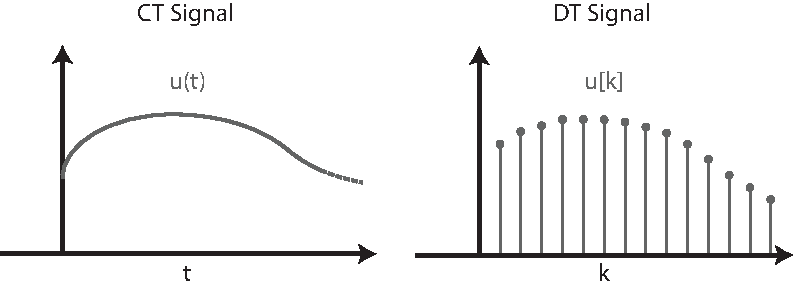
\includegraphics[width=0.9\textwidth]{signals}
    \caption{CT vs DT Signal}
\end{figure}

\subsubsection*{$\infty$-norm}

In the chacarterization and analysis of input-output stability of linear dynamical systems, most commonly 
used norm concept is the $\infty$-norm which is technically e measure of peak magnitude over time.
For scalar signals $\infty$-norm is defined as
%
\begin{align*}
	|| f ||_{\infty} &\triangleq \underset{k}{\sup}| f(k) | \quad (\mathrm{DT})
	\\
	&\triangleq \underset{t}{\sup}| f(t) | \quad (\mathrm{CT})
\end{align*}
%
The ``sup'' denotes the \textit{supremum} or \textit{least upper bound}, the value
that is approached arbitrarily closely but never (i.e.,\ at any finite time) exceeded.
Note that this is the natural standard $\infty$-norm definition for finite-dimensional
vectors to the infinite dimensional case, i.e. DT and CtT signals. Let's remember 
the $\infty$-norm of an $n$-dimensional vector, 
%
\begin{align*}
|| v ||_{\infty} \triangleq \underset{i\in[1,n]}{\max} | v_i | \ , \ \mathrm{where} v \in \mathbb{R}^n , 
\end{align*}
% 
A scalar signal, $f(.)$ is called \textit{bounded} if $|| f ||_{\infty} = M < \infty$ and that is the
fundamental signal measure adopted in BIBO stability. 

For multi-variate signals, we add a ned ``dimension'' in addition to the
time dimension, thus in such a case we define $\infty$-norm as
%
\begin{align*}
	|| f ||_{\infty} &\triangleq \underset{k}{\sup}|| f(k) ||_{\infty} \quad (\mathrm{DT})
	\\
	&\triangleq \underset{t}{\sup}|| f(t) ||_{\infty} \quad (\mathrm{CT})
\end{align*}
%
The space of all signals with finite $\infty$-norm are generally denoted by 
$\ell_{\infty}$ and $\mathcal{L}_{\infty}$ for DT and CT signals respectively.
For multi-variate case, the dimension of the vector may be explicitly added 
as $\ell^n_{\infty}$ and $\mathcal{L}^n_{\infty}$.

$\infty$-norms of some example CT and DT uni-lateral signals (i.e. $t \geq 0$
and $k \geq 0)$
%
\begin{align*}
	f(t) = 1 \, , \, || f ||_{\infty} = 1  \quad &- \quad g[k] = 1 \, , \, || g ||_{\infty} = 1
	\\
	f(t) = t \, , \, || f ||_{\infty} = \infty \quad &- \quad g[k] = k \, , \, || g ||_{\infty} = \infty
		\\
	f(t) = e^t \, , \, || f ||_{\infty} = \infty \quad &- \quad g[k] = 2^k \, , \, || g ||_{\infty} = \infty
			\\
	f(t) = 1 - e^t \, , \, || f ||_{\infty} = 1 \quad &- \quad g[k] = 1 - 0.5^k \, , \, || g ||_{\infty} = 1
				\\
	f(t) = \delta(t) \, , \, || f ||_{\infty} = \infty \quad &- \quad g[k] = \delta[k] \, , \, || g ||_{\infty} = 1
\end{align*}

\subsubsection*{$2$-norm}

$2$-norm of a signal is the most fundamental measure of signal in optimal control theory and it can be
considered as the square root of the ``energy'' of the signal. For scalar signals $2$-norm is defined as
%
\begin{align*}
	|| f ||_{2} &\triangleq \left[ \sum\limits_k (f[k])^2 \right]^{\frac{1}{2}} \quad (\mathrm{DT})
	\\
	&\triangleq \left[ \int\limits_t (f[t])^2 dt \right]^{\frac{1}{2}}  \quad (\mathrm{CT})
\end{align*}
%
For multivariate signals, we adopt the inner product and obtain
%
\begin{align*}
	|| f ||_{2} &\triangleq \left[ \sum\limits_k (f[k])^T f[k] \right]^{\frac{1}{2}} = 
	\left[ \sum\limits_k || f[k] ||_2^2 \right]^{\frac{1}{2}} 
	\quad (\mathrm{DT})
	\\
	&\triangleq \left[ \int\limits_t (f(t))^T f(t)  dt \right]  = 
	\left[ \sum\limits_k || f(t) ||_2^2 \right]^{\frac{1}{2}} 
	\quad (\mathrm{CT})
\end{align*}
%

% **** This ENDS THE EXAMPLES. DON'T DELETE THE FOLLOWING LINE:
\end{document}